% Results of the live experiment. Numbers come from generated/results.tex (analysis/make_figures.py).

\subsection{Setup}

The pipeline ran on a laptop in Paris (Intel Core i7-1260P, 16 hardware threads, Windows 11) connected to a
university Wi-Fi network, with TimescaleDB, Prometheus and Grafana in Docker, on \ExperimentDate{} from
\ExperimentStart{} to \ExperimentEnd{} UTC. It followed BTC and ETH on Binance (trades and order books),
Coinbase and Kraken (trades). The experiment had three phases:
\begin{enumerate}[nosep]
  \item a \emph{baseline} run of \BaselineMinutes{} minutes, including a planned \emph{noisy-neighbour} phase of
        \NoisyMinutes{} minutes during which the test suite and a storage benchmark ran in a loop on the same
        machine, competing for CPU and for the database;
  \item a \emph{planned stop} of \StopMinutes{} minutes, to test recovery after a restart;
  \item a \emph{fault-injection} run, during which each feed was forcibly disconnected at exponentially
        distributed intervals (mean 2 minutes) and kept down for 1 to 20 seconds.
\end{enumerate}
The independent latency probe ran throughout. Two earlier attempts are worth mentioning because they shaped the
setup: the first was interrupted when the laptop went to sleep, and the second failed because the university
network filters port 9443, on which Binance's streams are usually documented; the pipeline now connects on
port 443. \Cref{tab:runs} summarises the data collected and \cref{fig:throughput} the activity of each venue.

\begin{table}[ht]
\centering
\caption{Trades stored per run, by exchange time. Recovered trades were missed by the websocket and fetched
from the venue's history.}
\label{tab:runs}
\small
% Generated by analysis/make_figures.py
\begin{tabular}{llrrr}
\toprule
Run & Venue & Trades stored & live & recovered \\
\midrule
baseline & Binance & 653\,619 & 653\,146 & 473 \\
 & Coinbase & 203\,373 & 203\,265 & 108 \\
 & Kraken & 16\,342 & 16\,342 & 0 \\
\midrule
chaos & Binance & 277\,634 & 39\,253 & 238\,381 \\
 & Coinbase & 94\,827 & 13\,462 & 81\,365 \\
 & Kraken & 7\,941 & 1\,155 & 6\,786 \\
\bottomrule
\end{tabular}

\end{table}

\begin{figure}[ht]
  \centering
  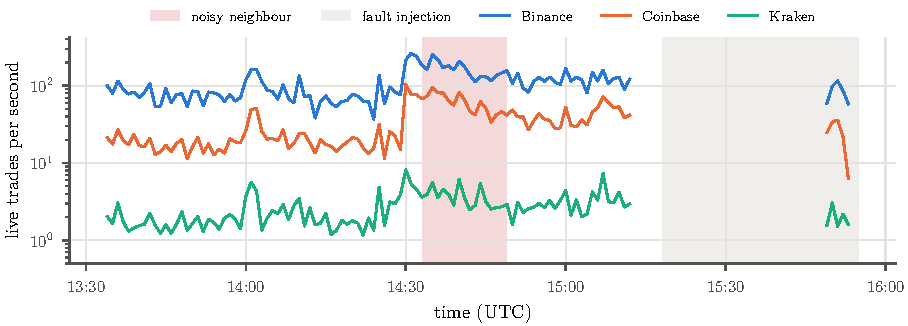
\includegraphics[width=\textwidth]{figures/throughput.pdf}
  \caption{Trades received live per second, per minute and venue (logarithmic scale). Shaded: the
  noisy-neighbour phase (red) and the fault-injection run (grey). The fault-injection run is interrupted by a
  26-minute suspension of the host, discussed in \cref{sec:res-losses}.}
  \label{fig:throughput}
\end{figure}

\subsection{Latency}\label{sec:res-latency}

\paragraph{Clock.} The first finding is about the local clock: during the whole experiment it was about
\emph{one second} ahead of UTC (\cref{fig:clock}). Over \NtpSamples{} NTP samples with a median round-trip
delay of \NtpDelayMedianMs\ms{}, the best samples put the offset between \NtpBestOffsetMinMs{} and
\NtpBestOffsetMaxMs\ms, drifting by \ClockDriftMsPerHour\ms{} per hour (\ClockDriftPpm{} ppm). Cristian's
algorithm on Binance's server time gives \BinanceRestOffsetMs\ms{} $\pm$ \BinanceRestUncMs\ms: an independent
confirmation, two orders of magnitude less precise because of the round trip to Tokyo. Without the
correction, every latency in this report would be overstated by a second, making Binance look ten times
slower than it is. The operating system's own synchronisation had not corrected this offset, which is common
on machines that synchronise rarely. Latencies below are corrected minute by minute; the uncertainty of the
correction over the quiet baseline is about $\pm$\QuietOffsetUncMs\ms.

\begin{figure}[ht]
  \centering
  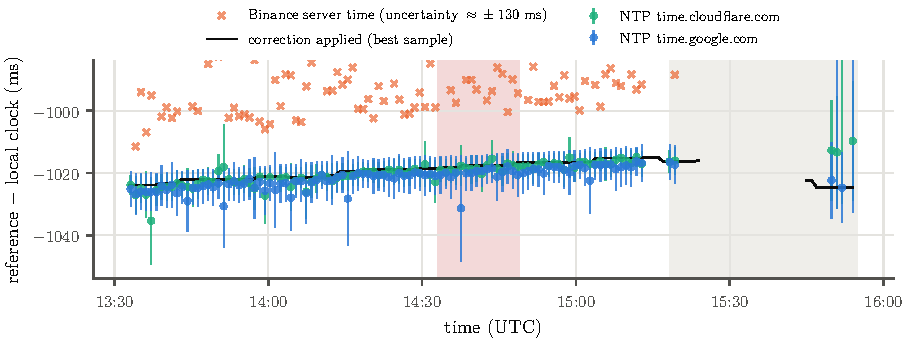
\includegraphics[width=\textwidth]{figures/clock.pdf}
  \caption{Offset of the local clock against two NTP servers (error bars: $\pm\delta/2$) and Binance's server
  time, and the correction applied to latencies.}
  \label{fig:clock}
\end{figure}

\paragraph{Exchange to receipt.} \Cref{tab:latency,fig:latency-cdf} give the distribution of the corrected
latency over the quiet part of the baseline (\QuietMinutes{} minutes). The minima are consistent with
geography: \LatBinanceMin\ms{} to Binance against a fibre bound of 48.6\ms{} (real routes to Tokyo are much
longer than the great circle), \LatCoinbaseMin\ms{} to Coinbase against 30.9\ms{}. Kraken, at
\LatKrakenMin\ms, is evidently served from much closer, presumably a European point of presence. The last
column, half the median round trip of websocket pings, estimates the one-way network delay without any clock.
It matches the latency minima for Coinbase (\RttCoinbaseHalf{} against \LatCoinbaseMin\ms) and Kraken
(\RttKrakenHalf{} against \LatKrakenMin\ms), which is a check of the clock correction itself. Binance answers
pings much more slowly than it streams data (\RttBinanceHalf\ms), so a ping-based estimate would be wrong there.

\begin{table}[ht]
\centering
\caption{Exchange time to receipt (ms), corrected for the local clock (about \QuietOffsetMs\ms), over the quiet
baseline, and half the median websocket ping round trip.}
\label{tab:latency}
\small
% Generated by analysis/make_figures.py
\begin{tabular}{lrrrrrrrrr}
\toprule
Venue & Trades & min & p1 & p50 & p90 & p99 & p99.9 & max & ping RTT/2 \\
\midrule
Binance & 309\,280 & 111.9 & 114.4 & 119.3 & 136.4 & 379 & 683 & 1675 & 198.3 \\
Coinbase & 81\,178 & 44.7 & 47.1 & 57.0 & 107.4 & 221 & 300 & 515 & 44.4 \\
Kraken & 7\,858 & 8.9 & 10.2 & 15.2 & 26.4 & 63 & 168 & 1189 & 9.6 \\
\bottomrule
\end{tabular}

\end{table}

\begin{figure}[ht]
  \centering
  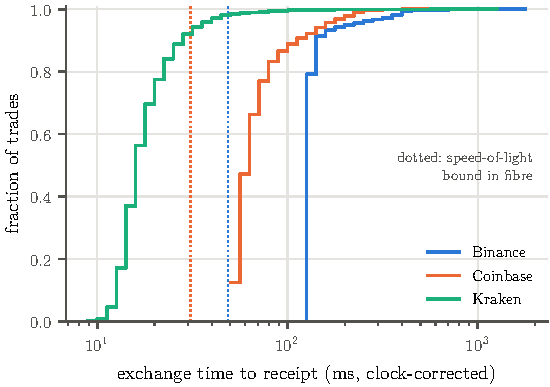
\includegraphics[width=0.62\textwidth]{figures/latency_cdf.pdf}
  \caption{Distribution of the corrected latency over the quiet baseline; dotted lines are the speed-of-light
  bounds in fibre.}
  \label{fig:latency-cdf}
\end{figure}

\begin{figure}[ht]
  \centering
  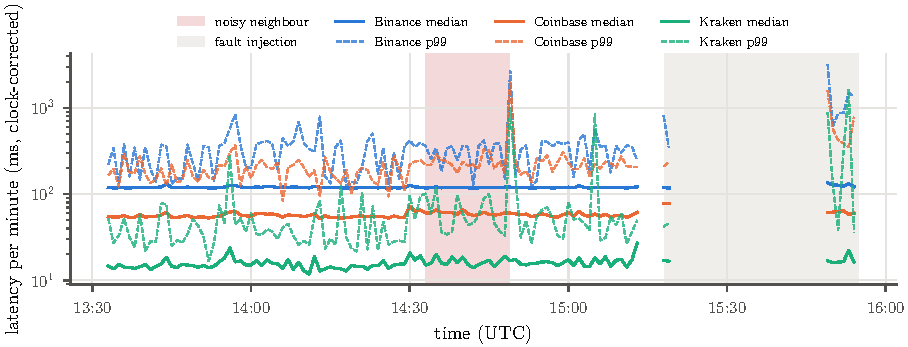
\includegraphics[width=\textwidth]{figures/latency_time.pdf}
  \caption{Median and 99th percentile of the corrected latency, per minute, over the whole experiment.}
  \label{fig:latency-time}
\end{figure}

The medians are stable to within a few milliseconds for two hours (\cref{fig:latency-time}), but the tails are long: the 99th
percentile is \LatBinancePninetynine\ms{} for Binance, \LatCoinbasePninetynine\ms{} for Coinbase and
\LatKrakenPninetynine\ms{} for Kraken, three to four times the median. They occur in bursts of trading, when a
venue publishes hundreds of messages within a few milliseconds.

\paragraph{Where the delay comes from.} Binance's event time $E$ separates its internal delay from transport:
the median of $E - T$ is \EminusTMedianMs\ms{} (maximum \EminusTMaxMs\ms), so Binance publishes trades almost as
soon as they happen and the tail arises between publication and receipt. To locate it, the independent probe
recorded the same quantity $t_{\mathrm{rx}} - E$ for BTC-USDT in a separate process (\cref{fig:probe}). The two
agree closely: over the \ProbeQuietSeconds{} seconds of the quiet baseline, the pipeline's per-second median
exceeds the probe's by \ProbeQuietDiffMedianMs\ms{} in the median, and most spikes appear in both series, which
places them upstream, in the network or in Binance's distribution layer. The tails differ, however: the
pipeline's excess reaches \ProbeQuietDiffPninetynineMs\ms{} at the 99th percentile, and it saw
\ProbeQuietPipeOverHalfSec{} seconds with a median above 500\ms{} against \ProbeQuietProbeOverHalfSec{} for
the probe.

The planned noisy-neighbour phase was meant to test whether this excess comes from competition for the CPU.
It does not: while the tests and the benchmark ran, the pipeline's excess over the probe was \emph{smaller}
(\ProbeNoisyDiffPninetynineMs\ms{} at the 99th percentile), its event-loop lag was unchanged
(\LoopLagNoisyPninetynine\ms{} at the 99th percentile, against \LoopLagQuietPninetynine\ms{} when quiet), and so
was its internal latency (\cref{tab:internal}). On a 16-thread machine, a load of this size leaves the pipeline
unaffected. The difference that remains between the two receivers is what they subscribe to: the probe receives
one trade stream, while the pipeline's Binance connection also carries two order book streams, which weigh far
more. During a burst, trades queue behind order book updates on the same TCP connection. The observations are
consistent with this head-of-line blocking, although the experiment does not isolate it; the design consequence
is that latency-critical streams belong on dedicated connections.

\begin{figure}[ht]
  \centering
  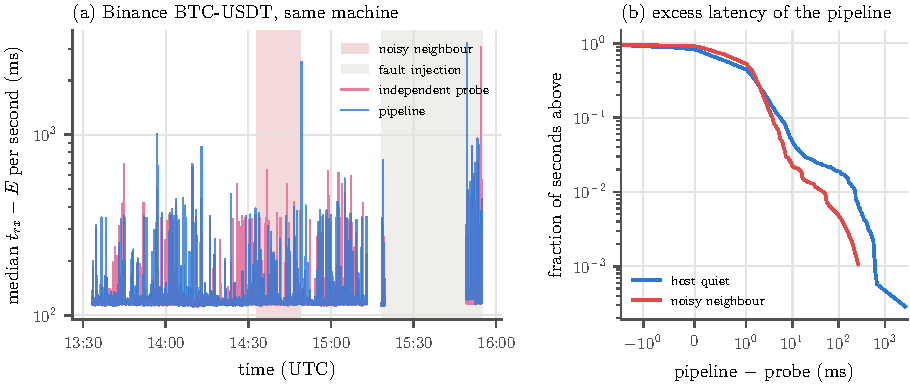
\includegraphics[width=\textwidth]{figures/probe.pdf}
  \caption{Control experiment. (a) Per-second median of $t_{\mathrm{rx}} - E$ for Binance BTC-USDT, measured by
  the pipeline and by an independent minimal receiver on the same machine. (b) Distribution of the pipeline's
  excess over the probe, per second, in the quiet baseline and during the noisy-neighbour phase.}
  \label{fig:probe}
\end{figure}

\subsection{Message loss and recovery}\label{sec:res-losses}

\Cref{tab:gaps} lists every gap. During the \BaselineMinutes{} minutes of the baseline no feed disconnected and
no sequence number was missed. The planned stop produced one restart gap per instrument, \RestartMissing{}
trades in total, all recovered at start-up.

During fault injection the pipeline was disconnected \ChaosDisconnects{} times, for a median of
\ChaosDowntimeMedianS{} seconds; each disconnection produced a gap whose size grows with the time disconnected
and with the venue's activity (\cref{fig:gaps}), and every gap was repaired. The most severe fault, however,
was not injected: at \SuspensionStart{} the host was suspended for \SuspensionMinutes{} minutes. Nothing was
logged during that interval although reconnections are retried at least every 30 seconds, so the process was
not running. On resumption, the feeds failed to connect for a few seconds until the network was back, then
reconnected and detected \SuspensionMissing{} missing trades, including a single gap of \LargestGap{} trades
on \LargestGapWhere. All of them were recovered from the venues' histories within three minutes.

Overall the pipeline detected \TotalMissing{} missing trades and recovered \TotalRecovered{}
(\RecoveredPctText). No gap was ever detected inside a connection, as expected over TCP. The median time from
detection to repair was \RepairMedianS{} seconds, of which one second is a deliberate wait that lets the REST
history catch up with the stream. On the order book side, \BookResyncs{} broken update chains, all after
reconnections, triggered a rebuild from a snapshot; none of the \QuotesStored{} best quotes stored was crossed.

\begin{table}[ht]
\centering
\caption{Sessions ended, gaps by cause, trades missed and recovered, and order book resyncs, per run and venue.}
\label{tab:gaps}
\small
% Generated by analysis/make_figures.py
\begin{tabular}{llrrrrrrr}
\toprule
Run & Venue & Disconn. & \multicolumn{3}{c}{Trade gaps} & Missed & Recovered & Book \\
\cmidrule(lr){4-6}
 & & & in session & reconnect & restart & trades & trades & resyncs \\
\midrule
baseline & Binance & 0 & 0 & 0 & 0 & 0 & 0 & 0 \\
 & Coinbase & 0 & 0 & 0 & 0 & 0 & 0 & 0 \\
 & Kraken & 0 & 0 & 0 & 0 & 0 & 0 & 0 \\
\midrule
chaos & Binance & 3 & 0 & 6 & 2 & 285\,964 & 285\,964 & 6 \\
 & Coinbase & 7 & 0 & 14 & 2 & 97\,344 & 97\,344 & 0 \\
 & Kraken & 4 & 0 & 8 & 2 & 8\,149 & 8\,149 & 0 \\
\bottomrule
\end{tabular}

\end{table}

\begin{figure}[ht]
  \centering
  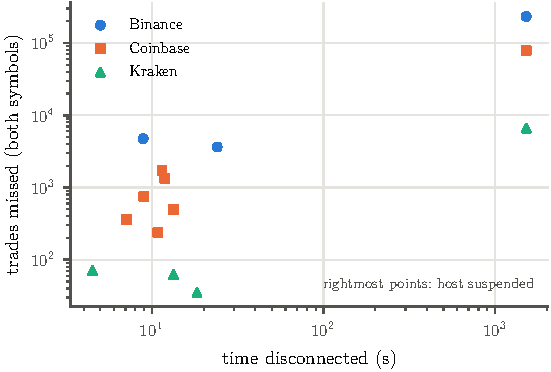
\includegraphics[width=0.62\textwidth]{figures/gaps_downtime.pdf}
  \caption{Fault-injection run: trades missed against the time disconnected, per venue. The rightmost points
  are the 26-minute host suspension.}
  \label{fig:gaps}
\end{figure}

The suspension also illustrates the difference between metrics and records. Prometheus ran in the same
suspended virtual machine and the counters restart with the process, so the dashboard's ``trades missed''
panel undercounts these events; the \code{gaps} table, written by the pipeline, has the exact count. Metrics are
for alerting; the database is the ledger.

\paragraph{Independent audit.} Sequence checks can only find what the pipeline knows to look for. The audit
compares every stored trade with the venue's own history for the same id range, per run and instrument
(\cref{tab:audit}). Out of \AuditReference{} trades in the venues' histories, \AuditMissing{} were missing from
the database, \AuditUnexpected{} were in the database but not in the history, and \AuditMismatched{} differed
in price, quantity, side or time; \AuditRecovered{} of the stored trades had been recovered by the backfill.

\begin{table}[ht]
\centering
\caption{Completeness audit against each venue's REST history (first and last minute of each run excluded).}
\label{tab:audit}
\small
% Generated by analysis/make_figures.py
\begin{tabular}{lllrrrrrr}
\toprule
Run & Venue & Symbol & Reference & Stored & Recovered & Missing & Extra & Altered \\
\midrule
baseline & Binance & BTC-USDT & 349\,886 & 349\,886 & 0 & 0 & 0 & 0 \\
 & Binance & ETH-USDT & 289\,343 & 289\,343 & 0 & 0 & 0 & 0 \\
 & Coinbase & BTC-USD & 164\,668 & 164\,668 & 0 & 0 & 0 & 0 \\
 & Coinbase & ETH-USD & 34\,583 & 34\,583 & 0 & 0 & 0 & 0 \\
 & Kraken & BTC-USD & 12\,326 & 12\,326 & 0 & 0 & 0 & 0 \\
 & Kraken & ETH-USD & 3\,777 & 3\,777 & 0 & 0 & 0 & 0 \\
\midrule
chaos & Binance & BTC-USDT & 135\,875 & 135\,875 & 122\,750 & 0 & 0 & 0 \\
 & Binance & ETH-USDT & 128\,998 & 128\,998 & 115\,423 & 0 & 0 & 0 \\
 & Coinbase & BTC-USD & 75\,432 & 75\,432 & 68\,030 & 0 & 0 & 0 \\
 & Coinbase & ETH-USD & 14\,046 & 14\,046 & 12\,839 & 0 & 0 & 0 \\
 & Kraken & BTC-USD & 5\,295 & 5\,295 & 4\,871 & 0 & 0 & 0 \\
 & Kraken & ETH-USD & 2\,073 & 2\,073 & 1\,865 & 0 & 0 & 0 \\
\bottomrule
\end{tabular}

\end{table}

\subsection{Pipeline internals and storage}

\Cref{tab:internal} gives the latencies inside the pipeline, on the monotonic clock. A trade reaches the
database \IngestQuietPfifty\ms{} after receipt in the median and \IngestQuietPninetynine\ms{} at the 99th
percentile, mostly the batching delay (a batch waits up to 100\ms{} for more rows) plus the write itself.
Decoding a Binance message takes about \ParseBinancePfiftyUs\,$\mu$s. The median event-loop lag of a few
milliseconds reflects the 15.6\ms{} timer resolution of Windows rather than load.

\begin{table}[ht]
\centering
\caption{Internal latencies (ms), from Prometheus histograms, per analysis window (the fault-injection window
excludes the suspension).}
\label{tab:internal}
\small
% Generated by analysis/make_figures.py
\begin{tabular}{lrrrrrr}
\toprule
Stage (ms) & \multicolumn{2}{c}{quiet baseline} & \multicolumn{2}{c}{noisy neighbour} & \multicolumn{2}{c}{fault injection} \\
\cmidrule(lr){2-3}\cmidrule(lr){4-5}\cmidrule(lr){6-7}
 & p50 & p99 & p50 & p99 & p50 & p99 \\
\midrule
Receipt to commit, trades & 125 & 318 & 126 & 298 & 132 & 422 \\
Receipt to commit, quotes & 104 & 262 & 107 & 274 & 114 & 337 \\
Batch write (COPY + insert) & 18.2 & 93.4 & 19.5 & 97.3 & 20.9 & 115 \\
Event loop lag & 6.49 & 24.2 & 5.78 & 24.1 & 6.43 & 24.7 \\
\bottomrule
\end{tabular}

\end{table}

The write path was benchmarked separately on 100\,000 synthetic trades (\cref{tab:storage}). The COPY-based
path is up to \BenchSpeedupMax{} times faster than \code{executemany} and reaches about \BenchBestRowsPerS{} rows
per second; replaying rows already stored is faster still, so idempotency costs little. The bottleneck is
index maintenance and continuous-aggregate invalidation on the hypertable; the deduplicating anti-join takes a
few milliseconds per batch. This capacity is about \CapacityRatio{} times the busiest minute observed
(\BusiestTradesPerS{} trades per second across all venues). Compressed, the
\TradesRows{} trades of the experiment occupy \TradesMBCompressed{} MB instead of \TradesMBUncompressed{} MB
(ratio \CompressionRatio), about \BytesPerTradeCompressed{} bytes per trade.

\begin{table}[ht]
\centering
\caption{Write throughput (rows per second) of the two insert strategies, on fresh rows and on a full replay
of rows already stored.}
\label{tab:storage}
\small
% Generated by analysis/make_figures.py
\begin{tabular}{rrrrr}
\toprule
Batch & \multicolumn{2}{c}{COPY + deduplicating insert} & \multicolumn{2}{c}{executemany} \\
\cmidrule(lr){2-3}\cmidrule(lr){4-5}
rows & new rows/s & replay rows/s & new rows/s & replay rows/s \\
\midrule
100 & 3\,976 & 7\,282 & 1\,480 & 1\,970 \\
1\,000 & 11\,646 & 16\,485 & 3\,720 & 3\,890 \\
10\,000 & 11\,092 & 93\,594 & 2\,990 & 3\,132 \\
\bottomrule
\end{tabular}

\end{table}
